\section{Alberi}
La definizione formale di albero sarà data quando tratteremo i grafi. Per ora 
diciamo che gli alberi sono strutture formate da nodi, simili alle liste, ma
con una rappresentazione gerarchica dei dati.
\begin{wrapfigure}{r}{7cm}
    \caption{Esempio di albero binario}
    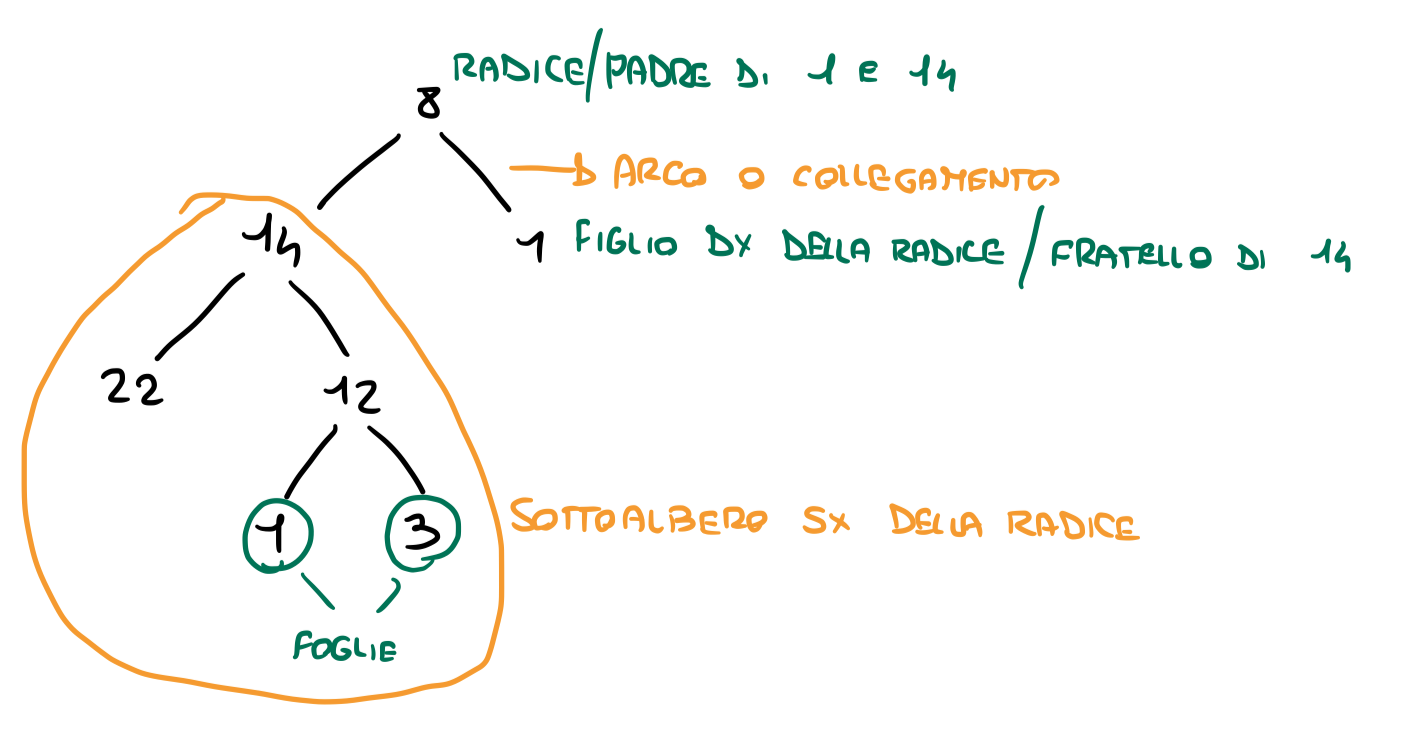
\includegraphics[scale = 0.3]{albero.png}
\end{wrapfigure}
La \emph{radice} è il nodo che sta in cima alla gerarchia. Ogni nodo ha un solo nodo 
{\emph{padre}} ma può avere un qualsiasi numero di \emph{figli}. La radice non ha un nodo padre.
I nodi che si trovano al livello più basso della gerarchia (i nodi che non hanno figli) sono detti
\emph{foglie}.
I collegamenti tra nodi sono detti \emph{archi}.\\
Un albero in cui ogni nodo può avere al massimo due figli è detto \emph{albero binario}
Possiamo dare una definizione ricorsiva di albero:\\
Un \textbf{albero binario} è:
\begin{itemize}
    \item una struttura vuota\\
    oppure 
    \item un nodo (radice) con associati due alberi binari detti \emph{sottoalbero sinistro} e \emph{sottoalbero destro}.
\end{itemize}
La radice di un albero ha \emph{profondità} pari a 0, i nodi di profondità $k$ 
hanno profondità $k + 1$.\\
Si definisce {\emph{altezza}} di un albero la massima profondità dei nodi.\\
Il \emph{grado} di un nodo è il massimo di figli che può avere quel nodo.\\
Alcuni esempi di dati rappresentati tramite alberi possono essere l'indice di un 
libro, uno schema del regno animale ma anche operazioni aritmetiche e in informatica
le chiamate ricorsive.
\subsection{Rappresentazione di alberi}
\subsubsection{Vettore dei padri}
\begin{figure}[h]
    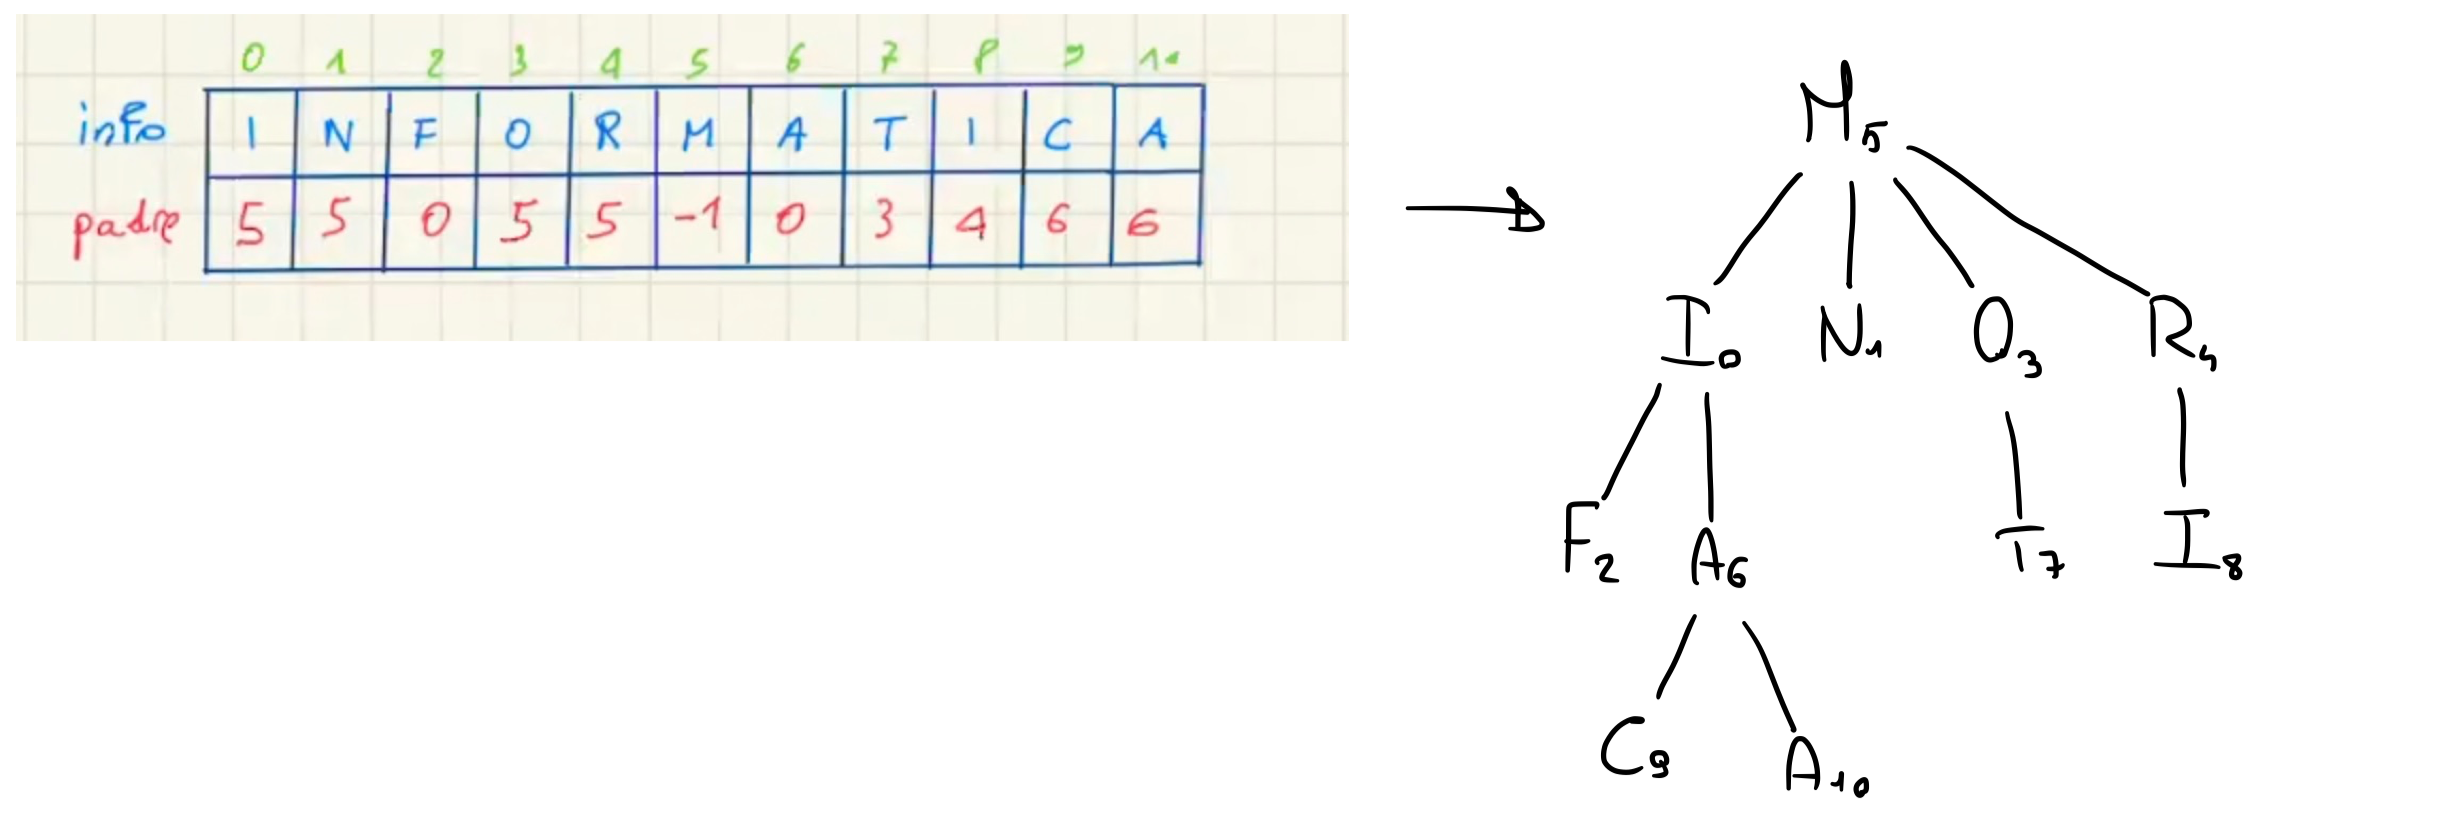
\includegraphics[width=\textwidth]{vettore_padri.png}
\end{figure}
\clearpage

\subsubsection{Rappresentazioni collegate: puntatori ai figli e lista dei fratelli}
\begin{figure}[h]
    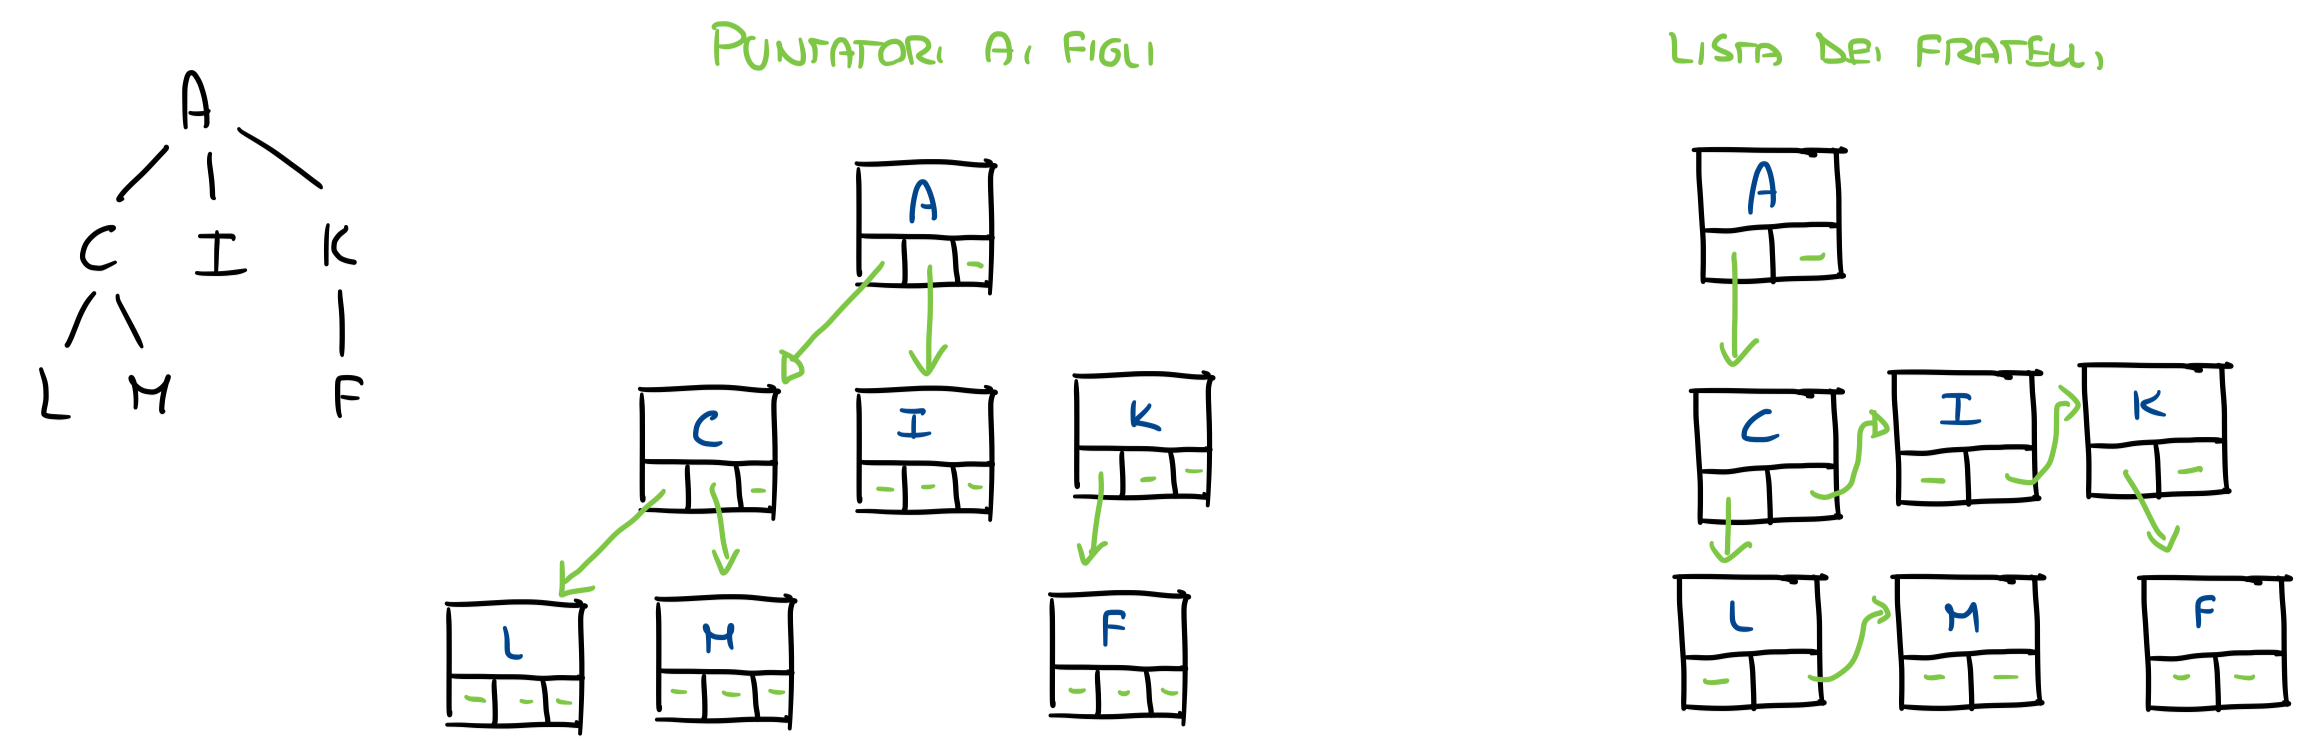
\includegraphics[width=\textwidth]{lista_fratelli.png}
\end{figure}

\subsection{Visite di alberi}
Vediamo ora alcune strategie per attraversare tutti i nodi di un albero.
\begin{algorithm}
    \caption{Visita generica}
    \Indm\textbf{Algoritmo} \emph{visitaGenerica}(\emph{AlberoBinario r})\\
    \Indp$S$ $\leftarrow$ $\lbrace r \rbrace$\\
    \While{$S \neq \emptyset$}{
        preleva un nodo $v$ da $S$\\
        visita $v$\\
        $S$ $\leftarrow$ $S$ $\cup$ $\lbrace$ figli di $v$ $\rbrace$
    }
\end{algorithm}

\begin{algorithm}
    \caption{Visita in ampiezza}
    \Indm\textbf{Algoritmo} \emph{visitaAmpiezza}(\emph{AlberoBinario r})\\
    \Indp$C$ $\leftarrow$ coda vuota\\
    $C.enqueue(r)$\\
    \While{\textbf{not} $C$.isEmpty()}{
        $n$ $\leftarrow$ $C.dequeue$\\
        \If{$n \neq null$}{
            visita il nodo associato a $n$\\
            $C.enqueue$($n.sx$)\\
            $C.enqueue$($n.dx$)\\
        }
    }
\end{algorithm}

\begin{algorithm}
    \caption{Visita in profondità}
    \Indm\textbf{Algoritmo} \emph{visitaProfondità}(\emph{AlberoBinario r})\\
    \Indp$P$ $\leftarrow$ pila vuota\\
    $P.push(r)$\\
    \While{\textbf{not} $P$.isEmpty()}{
        $n$ $\leftarrow$ $P.pop$\\
        \If{$n \neq null$}{
            visita il nodo associato a $n$\\
            $P.push$($n.sx$)\\
            $P.push$($n.dx$)\\
        }
    }
\end{algorithm}

\begin{algorithm}
    \caption{Visita in ordine anticipato}
    \Indm\textbf{Algoritmo} \emph{visitaPreOrder}(\emph{AlberoBinario r})\\
    \Indp\If{$r \neq null$}{
        visita la radice\\
        \emph{visitaPreOrder(r.sx)}\\
        \emph{visitaPreOrder(r.dx)}\\
    }
\end{algorithm}

\begin{algorithm}
    \caption{Visita in ordine simmetrico}
    \Indm\textbf{Algoritmo} \emph{visitaInOrder}(\emph{AlberoBinario r})\\
    \Indp\If{$r \neq null$}{
        \emph{visitaPreOrder(r.sx)}\\
        visita la radice\\
        \emph{visitaPreOrder(r.dx)}
    }
\end{algorithm}

\begin{algorithm}
    \caption{Visita in ordine posticipato}
    \Indm\textbf{Algoritmo} \emph{visitaPreOrder}(\emph{AlberoBinario r})\\
    \Indp\If{$r \neq null$}{
        \emph{visitaPreOrder(r.sx)}\\
        \emph{visitaPreOrder(r.dx)}\\
        visita la radice
    }
\end{algorithm}

\begin{algorithm}
    \caption{Numero nodi di un albero}
    \Indm\textbf{Funzione} \emph{numeroNodi}(\emph{AlberoBinario r}) $\rightarrow intero$\\
    \Indp\eIf{$r = null$}{
        \Return{0}
    }
    {
        $nsx \leftarrow numeroNodi(r.sx)$\\
        $ndx \leftarrow numeroNodi(r.dx)$\\
        \Return{1 + $nsx$ + $ndx$}
    }
\end{algorithm}
\clearpage


